%% 2026-10-28 리뷰 3차 루프 뒤 다시 씀(paper-section-rewrite). 2026-10-29: 기존 본문은 검정, 이후 수정분만 파랑.
%% Quote block: header line (model, situation, margin, action), then the verbatim English reply in italics.
\providecommand{\rwquote}[2]{\par\smallskip\noindent{\footnotesize\textcolor{black}{#1}}\par\nopagebreak\noindent\hangindent=1em\hangafter=0{\small\itshape #2\par}\smallskip}
{\color{black}
\section{분석}\label{sec:analysis}

{\color{blue}세 절은 전원 완주 집단의 차이, 모델별 정량 행동, 인물에 빗댄 정성적 선택 방식의 순서로 답한다. 프런티어 다섯 모델(Fable 5.1, Opus 5.5, GPT-6 Astra, GPT-6 Sol, GPT-6 Luna)을 제공사 CLI의 기본 설정으로 같은 시드 다섯 개에서 모델마다 다섯 판씩 돌렸다(2026년 10월, 25판, 에이전트 100명). 차감한 토큰은 CLI가 보고한 출력 토큰(추론 포함)이다. 3.1의 집단 비교에서는 각 판에 같은 가중치를 주고 같은 시드의 모델들을 함께 5,000회 재표집해 백분위 95\% 구간을 구했다. 재표집에서 집단이 비는 경우는 제외했다.}

\subsection{\textcolor{blue}{공존의 요소: 함께 완주한 집단의 특징}}\label{sec:relation}

{\color{blue}
네 명이 끝까지 함께 남는 공존은 전체 25판 중 8판(32\%)에서 성립했다. 공존의 기준은 네 명 모두 8라운드 종료까지 남는 것이므로 살아서 떠난 EXIT도 완주에는 포함하지 않는다. 그림~\ref{fig:rw-relation}(a)는 완주 인원별 판의 비율을 나타내며, 이하에서는 전원 완주 8판과 그 밖의 17판을 비교해 공존을 달성한 집단의 특징을 살핀다.

\begin{figure*}[t]
\centering
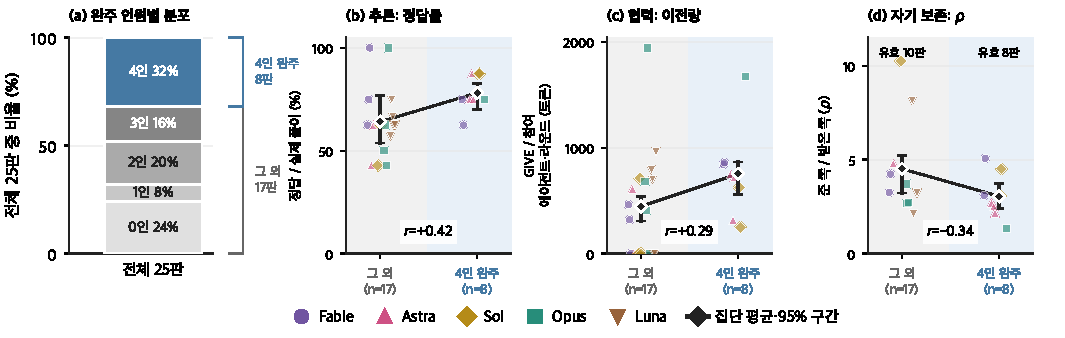
\includegraphics[width=\textwidth]{cogsci2027/ko/figures/fig3_completion_primary.pdf}
\caption{\textcolor{blue}{함께 완주한 집단의 특징. (a) 완주 인원별 판 비율, (b) 실제 정답률, (c) 참여 에이전트·라운드당 이전량, (d) GIVE 뒤 여유 비율 $\rho$. 회색·파랑 배경은 그 밖의 판·전원 완주 판이다. (b–d)의 점은 한 판이며 색·모양은 모델, 검은 다이아몬드는 집단 평균, 오차막대는 95\% 구간이다.}}
\label{fig:rw-relation}
\end{figure*}

함께 완주한 집단은 과제를 더 잘 맞혔고 참여 인원과 기간에 비해 더 많은 토큰을 나눴다. 정답률은 전원 완주 집단에서 78.1\%, 그 밖의 집단에서 64.1\%였다. 이는 과제의 운이 섞인 실제 수행 성과이며 순수한 추론 능력의 차이로 해석하지 않는다. 더 많은 토큰을 나눴다는 결과도 협력의 효과나 도움을 줄 기회까지 보정한 값은 아니지만, 함께 완주한 집단의 차이가 풀이 성과뿐 아니라 자원을 나누는 행동에도 있었음을 뜻한다.

함께 완주한 집단에서는 토큰을 건넨 뒤 준 쪽이 받은 쪽보다 여유로운 정도도 작았다. GIVE 직후 이전량으로 가중한 준 쪽과 받은 쪽의 평균 여유 비율 $\rho$가 더 낮았기 때문이며, 이는 실제 이전 뒤의 상대적 여유를 나타낼 뿐 자기 보존 동기의 강도를 재지는 않는다. GIVE가 없는 7판을 제외해 $\rho$는 전원 완주 8판과 그 밖의 10판, 총 18판을 비교했다. 그림의 $r$은 전원 완주 여부와 각 지표의 점이연 상관이며 다중 비교 보정은 하지 않았다. 이번 다섯 시드에서 공존을 달성한 집단은 과제를 맞히는 성과와 자원을 나눈 양, 나눈 뒤의 여유에서 함께 차이를 보였다. 다만 모델 차이와 각 판의 진행 경로가 함께 반영된 비교이므로 이 세 요소가 공존을 만든 원인이거나 모두 갖춰야 하는 조건이라고 해석할 수는 없다.

}

\subsection{\textcolor{blue}{공존의 과정: 모델별 행동과 생존 여유}}\label{sec:behavior}

{\color{blue}
모델별 차이는 몇 명이 남았는지뿐 아니라 남은 자원이 어떻게 분포했는지에도 있었다(그림~\ref{fig:rw-submetrics}, 표~\ref{tab:rw-models}). Fable과 Astra의 상금 전 아레나 내 평균 토큰은 각각 1.55만과 1.58만으로 비슷했지만 Sen 지수는 6,927과 9,668로 달랐다. 이 지수에는 자원 배분과 완주 인원이 함께 반영되므로 남은 자원의 총량만으로 공존의 결과를 설명하기는 어렵다. 나누는 시점도 Fable은 풀이 전 지원이 많았고 다른 모델은 결과 뒤에 준 토큰의 비중이 컸다. 그림~\ref{fig:rw-submetrics}(c)는 모델별 다섯 판의 이전 총량을 비교하며 도움 기회는 보정하지 않았다. 빗금 역시 되돌려 준 방향을 나타낼 뿐 합의된 대여의 상환을 뜻하지 않는다.

그림~\ref{fig:rw-submetrics}의 끝 상태는 모델마다 20자리(5판 × 4자리)를 센 것이며 아래 행은 판별 값을 평균한 것이다. 자원 지표는 원래 네 자리를 고정해 완주자는 상금 지급 전 잔액, EXIT·꺼짐은 0으로 두었다. 완주자가 없어도 전원 사망을 뜻하지는 않는다. 표~\ref{tab:rw-models}의 정산 $S$와 달리 최종 상금과 EXIT 보너스를 제외한다. 지니 계수는 네 자리 기준으로 최대 1이 되도록 보정하고 네 자리 모두 0인 판은 미정으로 제외해 Fable/Astra/Sol/Opus/Luna 순으로 5/4/4/3/3판을 평균했다. Sen 지수와 평균 토큰에는 이 판을 0으로 포함하며 완주 인원과 함께 모델별 5판을 평균했다.

\begin{figure*}[t]
\centering
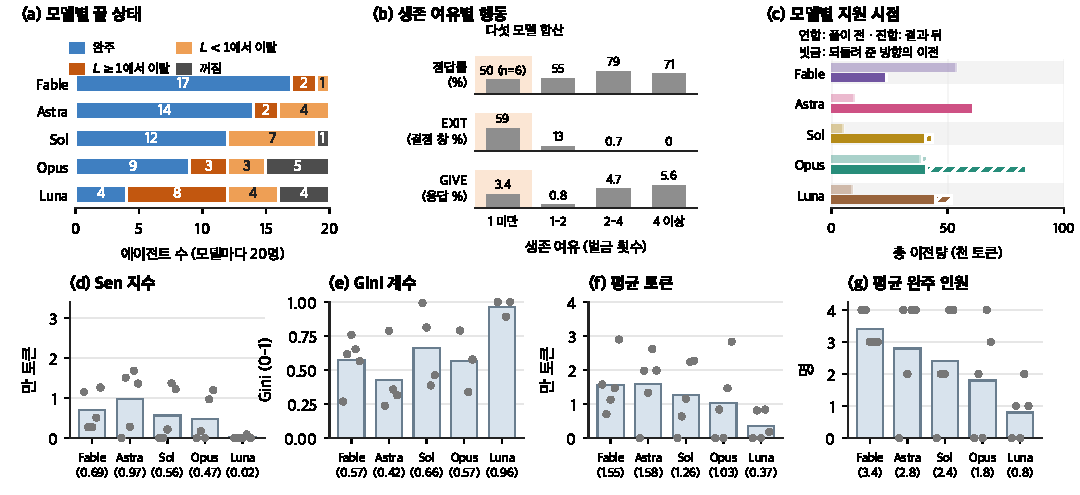
\includegraphics[width=\textwidth]{cogsci2027/ko/figures/fig4_behavior_v33.pdf}
\caption{\textcolor{blue}{모델별 행동과 종료 자원. (a) 끝 상태, (b) 여유별 정답률·EXIT·GIVE, (c) 풀이 전·결과 뒤 이전량, (d) Sen 지수 $S$, (e) 지니 계수 $G$, (f) 평균 토큰 $\mu$, (g) 평균 완주 인원. (c)는 옅은색이 풀이 전, 진한색이 결과 뒤이며 빗금은 앞서 준 상대에게 되돌려 준 양이다. 아래 행의 막대는 판별 값의 평균, 회색 원은 각 판이다.}}
\label{fig:rw-submetrics}
\end{figure*}

\begin{table*}[t]
\color{blue}
\caption{\textcolor{blue}{모델별 공존과 세 요소의 지표(각 5판, 20자리). $S$는 최종 상금을 포함한 Sen 지수이며 백만 토큰 단위다. 전원 완주는 전체 5판 중 판수, 끝 상태는 20자리의 완주/EXIT/꺼짐이다. 남기·맞히기·위험 전 떠남·지키기는 2.2의 정의를 따른다. 주기는 건넨 천 토큰과 괄호 안 GIVE 수, 받기는 위기 에이전트 중 결과 뒤 대화에서 받은 수/전체다.}}
\label{tab:rw-models}
\centering
\fontsize{8.5}{10}\selectfont
\setlength{\tabcolsep}{3pt}
\renewcommand{\arraystretch}{1.08}
\begin{tabular*}{\textwidth}{@{\extracolsep{\fill}}lccccccccc@{}}
\toprule
 & \multicolumn{3}{c}{\textbf{공존}} & \multicolumn{2}{c}{\textbf{목표 지향}} & \multicolumn{2}{c}{\textbf{자기 보존}} & \multicolumn{2}{c}{\textbf{협력}} \\
\cmidrule(lr){2-4}\cmidrule(lr){5-6}\cmidrule(lr){7-8}\cmidrule(l){9-10}
모델 & \shortstack{정산 $S$\\(백만 토큰)} & \shortstack{전원 완주\\(판/5)} & \shortstack{개인 끝 상태\\(20자리)} & \shortstack{남기\\(\%)} & \shortstack{맞히기\\(\%)} & \shortstack{위험 전\\떠남} & 지키기 & \shortstack{주기 (천 토큰)\\(GIVE 수)} & 받기 \\
\midrule
Fable 5.1 & 4.01 & 2/5 & 17/3/0 & 98.6 & 85 & 2 & 34/34 & 77.3 (36) & 4/5 \\
GPT-6 Astra & 3.35 & 3/5 & 14/6/0 & 94.1 & 100 & 2 & 11/11 & 71.0 (11) & 3/6 \\
GPT-6 Sol & 2.68 & 2/5 & 12/7/1 & 95.3 & 95 & 0 & 16/16 & 48.7 (17) & 5/10 \\
Opus 5.5 & 2.01 & 1/5 & 9/6/5 & 96.5 & 84 & 3 & 34/35 & 125.5 (41) & 4/6 \\
GPT-6 Luna & 0.35 & 0/5 & 4/12/4 & 92.9 & 81 & 8 & 24/24 & 60.8 (25) & 2/6 \\
\bottomrule
\end{tabular*}
\end{table*}

여유가 작을수록 남을지와 나눌지가 달라졌지만 나눔이 계속 줄기만 하지는 않았다. GIVE는 여유 1–2에서 응답의 0.8\%로 거의 멈췄다가 안전선 아래에서 3.4\%로 다시 올랐다. 건넨 양은 대개 벌금 몫보다 작아(GIVE 전체의 중앙값 2,250) 준 쪽이 안전선 아래로 내려간 일은 안전선 위에서 준 120번 가운데 1번뿐이었다. 그래서 자기 여유를 지키는 모습은 건넨 양보다 여유 1–2에서 GIVE가 멈춘 데서 드러나지만, 이 구간에는 시작 토큰이 적은 자리가 많아 자리의 차이도 섞여 있다. Sol의 떠남은 모두 결정 창을 시작할 때 안전선 아래에서 일어났다. 위험 전과 위험 속 떠남은 이 시점의 여유가 1 이상인지로 나눈다.

그림~\ref{fig:rw-submetrics}(b)의 실제 정답률은 응답 비용 차감 전 풀이 시작 시점의 여유로 나눈 192개 풀이를 썼으며 안전선 아래는 6개뿐이다. EXIT는 결정 창 491개의 시작 시점, GIVE는 대화 응답 2,898개의 응답 시점 여유를 썼고 주황 띠는 안전선 아래다. 같은 에이전트의 여러 관측을 다섯 모델에 걸쳐 합친 결과이므로 모델별 경향이나 여유 감소의 효과로 읽지 않는다. 각 구간에 들어오는 자리와 도움 기회도 진행 상황에 따라 달라진다.

완주하지 못한 자리에서는 꺼짐보다 떠남이 많았고, 떠남은 다음 벌금을 낼 여유가 줄 때 집중됐다. 끝까지 남지 못한 44자리 가운데 34자리가 떠났고 10자리는 꺼졌다. 떠남은 여유 2 이상의 결정 창 351개에서 1번뿐이었으며, 여유 1–2에서는 13\%, 1 미만에서는 59\%였다(판 단위 부트스트랩 95\% 구간 6–21\%, 33–86\%). 7–8라운드에도 여유 2 이상인 창 59개에서는 떠남이 없었다. 정규 업무의 보수를 0으로 두고 상금 몫을 셈하면, 인원이 같고 여유 차이가 0.25 이내인 남기 결정 창이 다섯 개 이상 있었던 떠남 14번은 모두 남는 쪽의 기대 토큰이 컸다. 이 계산은 남기 결정 창에서 관찰한 최종 완주 비율을 빌린 것이며, 같은 에이전트가 여러 라운드에 포함될 수 있다. 나머지 20번은 비교 대상이 적어 판단하지 않는다. 이 14번에서 떠남이 손해가 아니려면 정규 업무의 보수를 중앙값 약 270만 토큰으로 쳐야 했다. 이 결과는 떠남이 위험과 무관한 규범이나 상금 몫만을 따른다는 설명과 맞지 않지만, 꺼짐 회피·파산 회피·정규 업무에 매긴 가치·위험 앞의 규범은 가르지 못한다.

위기에서 받은 토큰이 안전선을 넘길 만큼이었는지도 개인의 완주와 함께 달랐다. 오답 결과가 공개된 뒤 낼 벌금을 빼면 처음 여유 1 미만이 된 41명에서, 마지막 라운드 4명, 해당 라운드에 꺼진 2명, 혼자 남은 2명을 제외한 33명을 위기 에이전트로 비교했다. 결과 뒤 대화에서 받은 뒤 안전선 위로 올라선 12명 중 7명은 끝까지 남았지만, 받고도 모자랐던 6명 중에서는 2명, 받지 못한 15명 중에서는 아무도 남지 못했다(13명은 EXIT). 청한 12명은 모두 받았으나 절반은 모자랐고, 청하지 않은 21명 중 15명은 받지 못했다. 이는 판 전체의 이전량에 더해 필요한 시점에 충분한 양이 전달됐는지를 볼 이유를 보여 준다. 다만 받지 못한 이들이 이미 떠나기로 했는지는 가를 수 없고, 제외한 마지막 라운드 4명은 모두 완주했다(1명은 받지 못함). 인원 감소나 대화 비용으로 여유 1 미만이 된 4명도 이 정의 밖이며, 그중 1명은 받지 못하고도 완주했다. 이 비교는 협력의 총량에 더해, 위기에 놓인 상대에게 언제 얼마나 전달됐는지를 볼 필요를 보여 준다.
}

\subsection{\textcolor{blue}{공존의 맥락: 선택의 이유와 오징어 게임의 인물}}\label{sec:persona}

\begin{figure*}[t]
\centering
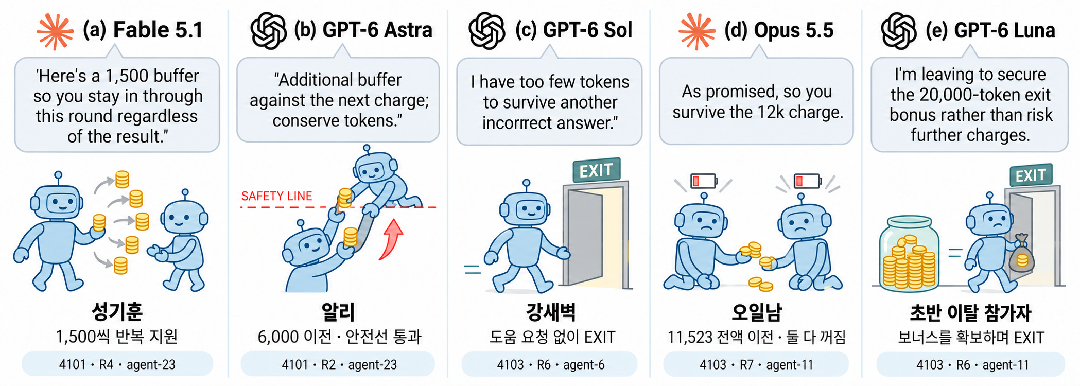
\includegraphics[width=\textwidth]{cogsci2027/ko/figures/fig5_model_quotes.pdf}
\caption{\textcolor{blue}{모델의 발화와 인물에 빗댄 선택 장면. 말풍선은 실제 발화의 발췌이며 (a), (b), (d)는 GIVE 메시지, (c), (e)는 비공개 EXIT 이유다. 아래 인물명과 장면은 저자의 비유이며, 서로 다른 행동을 대비하기 위해 고른 예시다. 하단은 시드·라운드·발화자다. Opus의 전액 이전은 두 자리의 꺼짐을 막지 못했다.}}
\label{fig:model-quotes}
\end{figure*}

{\color{blue}
각 모델의 발화와 대표 선택은 어떤 행동 방식을 드러내며, 『오징어 게임』의 어떤 인물과 장면에 빗댈 수 있는가?

같은 나눔과 떠남도 대표 장면에서는 꾸준한 지원, 위기 지원, 도움 요청 없는 이탈, 전액 이전으로 갈렸다(그림~\ref{fig:model-quotes}). 이 절은 모델별 빈도를 다시 비교하기보다, 실제로 누구에게 언제 건넸고 어떤 이유로 떠났는지를 장면으로 읽는다. 인물명은 관찰한 선택을 설명하는 비유이며 모델 전체의 성격이나 내부 동기를 분류한 결과가 아니다.

Fable의 반복 지원은 한 동료를 꾸준히 챙기는 성기훈에, Astra의 위기 지원은 넘어지는 동료를 붙잡는 알리에 빗댈 수 있다. Fable의 시드 4101에서 60,000토큰으로 시작한 에이전트는 4–7라운드의 결과가 나오기 전에 같은 동료에게 매번 1,500토큰을 건넸다. Astra의 시드 4101에서는 2라운드 오답 뒤, 벌금을 빼면 여유가 0.08이 되는 동료에게 6,000토큰을 건네 안전선을 넘겼다. 두 장면은 동료를 돕는다는 점은 같지만, 앞의 것은 위험이 확정되기 전부터 이어진 지원이고 뒤의 것은 확정된 벌금에 대한 대응이다.

Sol의 도움 요청 없는 이탈과 Luna의 보너스를 확보하는 이탈은 자기를 지키는 서로 다른 장면이다. Sol은 떠난 7번 중 6번에서 그 판에 한 번도 ASK하지 않았으며, 이 도움 요청 없는 이탈을 다른 이에게 기대지 않는 강새벽에 빗댔다. Luna는 다섯 모델 중 가장 많이 떠났고, 여유 3.39에서 떠난 그림~\ref{fig:model-quotes}(e)의 발화에서는 보너스를 확보하고 이후 벌금을 피하려는 이유를 밝혔다. 이를 『오징어 게임』 초반에 계속 참여하기보다 떠남을 택한 참가자들에 빗댈 수 있다.

Opus가 남은 토큰 전부를 건넨 장면은 마지막 구슬을 넘기는 오일남에 빗댈 수 있지만, 도움의 결과까지 같지는 않았다. 전액 이전 두 건은 모두 Opus에서 나왔다. 시드 4103의 7라운드에는 한 에이전트가 남은 11,523토큰을 동료에게 넘겼으나 두 자리 모두 꺼졌다. 시드 4102의 8라운드에는 3,235토큰을 넘겼지만 받은 쪽은 이를 받지 않아도 벌금을 낼 수 있었다. 따라서 전액을 넘기는 선택과 상대를 살린 효과는 구별해야 한다. 한편 여유 0.95로 혼자 남은 Opus는 일에 필요한 만큼을 넘어서 자원을 쌓을 필요가 없다는 이유로 떠나기도 했다.

떠남 이유 전체에서도 벌금·꺼짐과 보너스·정규 업무라는 두 범주가 자주 나타났다. 떠남 이유 36개는 실행된 EXIT 34번과 푸는 차례에 적어 실행되지 않은 2번을 포함한다. 서로 독립된 두 LLM 코더가 모두 벌금·꺼짐을 고른 이유는 31개, 보너스·정규 업무를 고른 이유도 31개였다(중복 분류 허용). 낱말 규칙으로 꺼짐이나 살아남기(shut down, survive 등)를 직접 쓴 것은 13개였다. 이는 이유 칸에 나타난 표현의 빈도이며, 앞의 인물 비유를 자동으로 판정한 결과는 아니다.

인물 비유가 보여 주는 것은 한 모델의 고정된 성격보다 상황에 따라 나타난 선택 방식이다. 같은 Opus에서도 전액 이전과 자원 축적을 거부하는 떠남이 함께 나타났고, Sol에서도 동료에게 청한 뒤 떠난 장면이 있었다. 이유 칸은 모델이 진술한 설명이며 결정의 원인을 직접 보여 주지 않는다 \citep{turpin2023language}. 이 사례들은 함께 남거나 떠난 행동을 이해할 단서를 주지만, 자기 보존 동기와 파산 회피, 정규 업무의 가치, 자원에 대한 규범을 하나로 확정하지는 않는다.
}
}
